\documentclass{beamer}
\usepackage{caption}
\usepackage{float}
\usepackage{lscape}
\usepackage{graphicx}% http://ctan.org/pkg/graphicx
\usepackage{booktabs}% http://ctan.org/pkg/booktabs
\usepackage{array}
\usepackage[export]{adjustbox}
\usepackage{amsmath}
\usepackage{amsfonts}
\usepackage{amssymb}
\usepackage{tikz}
\usepackage{ upgreek }
\usepackage{subcaption}
\usepackage{tabularx} 
\usepackage{setspace}



\graphicspath{ {images/} }
\usetheme{Frankfurt}
%\usefonttheme{structuresmallcapsserif} 
\definecolor{Gold}{RGB}{218,165,32}
\setbeamertemplate{navigation symbols}{}
\setbeamertemplate{theorems}[numbered]
\setbeamertemplate{theorems}[ams style] 
%\setbeamertemplate{navigation symbols}{}

\renewcommand{\qedsymbol}{$\blacksquare$}
\makeatletter

\setbeamerfont{footline}{size=\fontsize{6}{8.5}\selectfont}

\defbeamertemplate*{footline}{Dan P theme}
{
  \leavevmode%
  \hbox{%
  \begin{beamercolorbox}[wd=.15\paperwidth,ht=2.25ex,dp=1ex,center]{author in head/foot}%
    \usebeamerfont{author in head/foot}\insertshortauthor\expandafter\beamer@ifempty\expandafter{\beamer@shortinstitute}{}{~~(\insertshortinstitute)}
  \end{beamercolorbox}%
  \begin{beamercolorbox}[wd=.63\paperwidth,ht=2.25ex,dp=1ex,center]{title in head/foot}%
    \usebeamerfont{title in head/foot}\insertshorttitle
  \end{beamercolorbox}%
  \begin{beamercolorbox}[wd=.22\paperwidth,ht=2.25ex,dp=1ex,right]{date in head/foot}%
    \usebeamerfont{date in head/foot}\insertshortdate{}\hspace*{1.5em}
\insertframenumber{} / \inserttotalframenumber\hspace*{4ex} 
  \end{beamercolorbox}}%
  \vskip0pt%
}

\makeatother

\title{Labor Risk and the Cross-section of Expected Returns \\ }

% many auto-annotations to stargazer tables are wrong, since 
% I usually copypasted tabular output into table environment
% from Nov 19 version.

\author{Mykola Pinchuk}

\date{01/08/2022}

\subject{Empirical Asset Pricing}

%\AtBeginSubsection[]
%\setcounter{section}{1}
\begin{document}

\begin{frame}
  \titlepage
\end{frame}

\section{Overview}
\subsection{}

\begin{frame}{Introduction}
\begin{itemize}
    \item {The economy has permanently evolving structure.}
    \item {Accelerated rate of sectoral reallocation creates unemployment risk for workers in declining industries.}
    \item {Many workers possess significant industry-specific skills.}
    \item {Sectoral shifts create large labor income risk for workers with industry-specific skills.}
    \item {Since employees can not fully hedge labor income risk, it should be relevant for asset pricing.}
    \item {\textbf{Is the rate of sectoral shifts a state variable?}}
\end{itemize}

\end{frame}


\begin{frame}{Key results}
\begin{itemize}
    \item {I use cross-industry dispersion (CID) to measure the rate of sectoral shifts.}
    \item {CID is the cross-sectional mean absolute deviation of the returns of industry portfolios.}
    \item {Stocks with high sensitivity to CID produce low returns.}
    \item {This return spread (49 bps) is not explained by common factors.}
    \item {Unlike CID, within-industry dispersion (WID) is not priced.}
    \item {Consistent with the hypothesis that CID proxies for labor risk from sectoral shifts, CID predicts unemployment.}
\end{itemize}
\end{frame}

\section{Literature}
\subsection{}

\begin{frame}{Literature}
\begin{itemize}
    \item {Theory:}
    \begin{itemize}
        \item {Constantinides and Duffie (1996).}
    \end{itemize}
    \item {Empirical papers on idiosyncratic risk:}
    \begin{itemize}
        \item {Ang, Hodrick, Xing and Zhang (2006).}
        \item {Herskovic, Kelly, Lustig and Van Nieuwerburgh (2016).}
        \item {Verousis and Voukelatos (2018): High sensitivity to cross-sectional dispersion (CSD) is related to low returns.}
    \end{itemize}
    \item {Macroeconomic literature on unemployment and sectoral shifts:}
    \begin{itemize}
        \item {Lilien (1982): Unemployment is driven by two forces: aggregate shocks and sectoral shifts.}
        \item {Loungani, Rush and Tave (1990), Brainard and Cutler (1993).}
    \end{itemize}
\end{itemize}
\end{frame}



\begin{frame}{Relationship to literature}
\begin{itemize}
    \item {Bridges the gap between macro and asset pricing literature on unemployment risk due to sectoral shifts. \\ Shows asset pricing implications of unemployment, driven by sectoral shifts.}
    \item {Provides evidence, broadly consistent with the model of Constantinides and Duffie (1996).}
    \item {Provides fundamental economic explanation for the cross-sectional returns predictability by CSD (Verousis and Voukelatos 2018).\\
    This predictability is driven by the cross-industry component of CSD (i.e., CID).}
\end{itemize}
\end{frame}


\section{Data and Key Results}
\subsection{}


\begin{frame}{Data}
\begin{itemize}
    \item {CRSP 1926-2019 and Compustat 1963-2019.}
    \item {Fama-French industry portfolios and factors from French`s website.}
    \item {Uncertainty indices from Ludvigson`s website.}
    \item {Unemployment and industry employment data from Bureau of Labor Statistics.}
\end{itemize}
\end{frame}



\begin{frame}{Cross-Industry Dispersion}
\begin{itemize}
    \item {Cross-Industry Dispersion (CID) is the mean absolute deviation of the returns of FF49 industries.}
    \item {I measure CID at the monthly frequency: \\
    $$CID_t = \frac{1}{N}\sum^{N}_{i=1}{|R_{it}-R_{MKT,t}|}.$$}
    \item {In every period, I use only the industries with at least 10 firms, so $N \leq 49$.}
    \item {I compute within-industry dispersion (WID) as the mean absolute deviation between stock returns and value-weighted return of its industry:
    $$WID_t = \frac{1}{N}\sum^{N}_{j=1}\frac{1}{M_j}\sum^{M_j}_{i=1}{|R_{it}-R_{jt}|}.$$}
\end{itemize}
\end{frame}



\begin{frame}{Time series of CID}
{Figure 1}
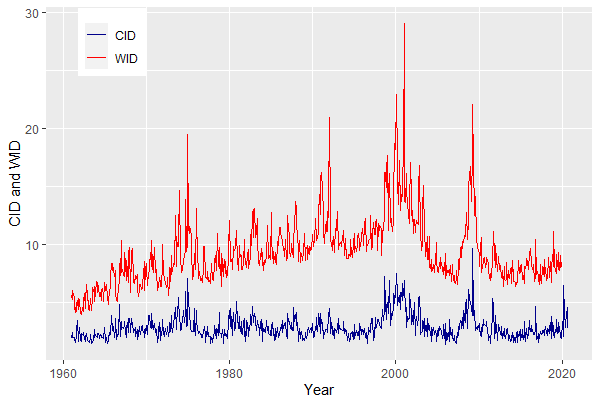
\includegraphics[width=1\textwidth]{paper_nov20/cid_wid_w.png}
\end{frame}



\begin{frame}{Cross-Industry Dispersion}
\begin{table}[!htbp] \centering 
  \caption*{\textbf{Table 1: Correlations of differences in CID with differences in other variables}} 
  \label{} 
    \begin{flushleft}
    {\medskip\scriptsize
 The table reports correlations between differences in CID and differences in other variables at the monthly frequency. FU and MU are financial and macroeconomic uncertainty from Sydney Ludvigson website. VOL is the volatility of monthly value-weighted market index over the recent 24 months. CIV is common idiosyncratic volatility (Herskovic et al., 2016). }
    \medskip
    \end{flushleft}
\small
\vspace{-0.1cm}
\begin{tabular}{@{\extracolsep{5pt}} ccccccc} 
\\[-1.8ex]\hline 
\hline \\[-1.8ex] 
 & CID & FU & MU & VOL & CIV & VIX \\ 
\hline \\[-1.8ex] 
CID & $1$ & $0.24$ & $0.07$ & $0.30$ & $0.29$ & $0.11$ \\ 
FU & $0.24$ & $1$ & $0.44$ & $0.30$ & $0.39$ & $0.40$ \\ 
MU & $0.07$ & $0.44$ & $1$ & $0.11$ & $0.24$ & $0.36$ \\ 
VOL & $0.30$ & $0.30$ & $0.11$ & $1$ & $0.27$ & $0.34$ \\ 
CIV & $0.29$ & $0.39$ & $0.24$ & $0.27$ & $1$ & $0.50$ \\ 
VIX & $0.11$ & $0.40$ & $0.36$ & $0.34$ & $0.50$ & $1$ \\ 
\hline \\[-1.8ex] 
\end{tabular} 
\end{table}
\end{frame}



\begin{frame}{Estimation of $\beta_{CID}$}
\begin{itemize}
    \item {I difference and residualize $CID_t$ using the specification from Pastor and Stambaugh (2003):
    $$\Delta(CID_t) = \gamma_0 + \gamma_1 \Delta(CID_{t-1}) + \gamma_2 CID_{t-1} + \widetilde{CID}_t.$$}
    \item {I use 2 years of monthly data to estimate $\beta_{CID}$ of every stock:
    $$R_{t}=\alpha+\beta \widetilde{CID}_t + \epsilon_t.$$}
    \item {Then I sort stocks into quintile portfolios according to $\beta_{CID}$.}
\end{itemize}
\end{frame}


\small
\begin{frame}{Returns of quintile portfolios, formed on $\beta_{CID}$}
\begin{table}[!htbp] \centering 
  \caption*{\textbf{Table 3: Returns of quintile $\beta_{CID}$-sorted portfolios}}
  \label{} 
  \vspace{-0.2cm}
\begin{tabular}{@{\extracolsep{2pt}} ccccccc} 
\\[-1.8ex]\hline 
\hline \\[-1.8ex] 
 & Q1 & Q2 & Q3 & Q4 & Q5 & L/S \\ 
\hline \\[-1.8ex] 
Mean ew & 0.81$^{***}$ & 0.79$^{***}$ & 0.73$^{***}$ & 0.65$^{***}$ & 0.50$^{**}$ & -0.31$^{**}$ \\ 
T-stat ew & 3.56 & 4.09 & 3.96 & 3.42 & 2.09 & -2.47 \\ 
Mean vw & 0.79$^{***}$ & 0.63$^{***}$ & 0.58$^{***}$ & 0.45$^{***}$ & 0.30 & -0.49$^{***}$ \\ 
T-stat vw & 3.83 & 3.51 & 3.55 & 2.59 & 1.40 & -3.19 \\ 
\hline \\[-1.8ex] 
\end{tabular} 
\end{table}

% Table created by stargazer v.5.2.2 by Marek Hlavac, Harvard University. E-mail: hlavac at fas.harvard.edu
% Date and time: 10/14
\begin{table}[!htbp] \centering 
  \caption*{\textbf{Table 4: Abnormal returns of quintile $\beta_{CID}$-sorted vw portfolios}} 
  \label{} 
  \vspace{-0.2cm}
\begin{tabular}{@{\extracolsep{0pt}} lcccccc} 
\\[-1.8ex]\hline 
\hline \\[-1.8ex] 
Statistic & Ret & $\alpha_{CAPM}$ & $\alpha_{FF3}$ & $\alpha_{Carhart}$ & $\alpha_{FF5}$ & $\alpha_{FF5+UMD+STR}$ \\ 
\hline \\[-1.8ex] 
L/S & -0.49$^{***}$ & -0.52$^{***}$ & -0.40$^{***}$ & -0.63$^{***}$ & -0.29$^{*}$ & -0.50$^{***}$ \\ 
 & [ -3.19] & [ -3.42] & [ -2.64] & [ -4.22] & [ -1.87] & [ -3.26] \\
\hline \\[-1.8ex] 
\end{tabular} 
\end{table}
\end{frame}


\small
\begin{frame}{Characteristics of quintile portfolios, formed on $\beta_{CID}$}
\begin{table}[!htbp] \centering 
  \caption*{\textbf{Table 2: Characteristics of quintile $\beta_{CID}$-sorted vw portfolios}} 
  \label{} 
\begin{tabular}{@{\extracolsep{5pt}} lcccccc} 
\\[-1.8ex]\hline 
\hline \\[-1.8ex] 
 & Q1 & Q2 & Q3 & Q4 & Q5 & L/S \\ 
\hline \\[-1.8ex] 
Return & $0.79$ & $0.63$ & $0.58$ & $0.45$ & $0.30$ & $$-$0.49$ \\ 
T-stat (Return) & $3.83$ & $3.51$ & $3.55$ & $2.59$ & $1.40$ & $$-$3.19$ \\ 
Prebeta & $$-$3.25$ & $$-$1.08$ & $0.27$ & $1.66$ & $4.12$ & $7.37$ \\ 
Size & $8.12$ & $8.76$ & $8.96$ & $8.87$ & $8.40$ & $0.28$ \\ 
log(B/M) & $$-$0.78$ & $$-$0.77$ & $$-$0.78$ & $$-$0.80$ & $$-$0.84$ & $$-$0.07$ \\ 
OP & $0.16$ & $0.17$ & $0.17$ & $0.17$ & $0.17$ & $0.01$ \\ 
Investment & $0.15$ & $0.15$ & $0.14$ & $0.15$ & $0.22$ & $0.08$ \\ 
Beta & $1.04$ & $0.98$ & $0.99$ & $1.03$ & $1.14$ & $0.11$ \\ 
BA Spread & $0.31$ & $0.23$ & $0.20$ & $0.19$ & $0.21$ & $$-$0.10$ \\ 
Momentum 12-2 & $0.12$ & $0.09$ & $0.10$ & $0.12$ & $0.19$ & $0.07$ \\ 
Volatility (1m) & $2.01$ & $1.68$ & $1.61$ & $1.69$ & $2.07$ & $0.06$ \\ 
Volatility (12m) & $2.13$ & $1.75$ & $1.69$ & $1.79$ & $2.21$ & $0.08$ \\ 
\hline \\[-1.8ex] 
\end{tabular} 
\end{table}
\end{frame}

\normalsize
\begin{frame}{Interpretation of $\beta_{CID}$}
\begin{itemize}
    \item {High-$\beta_{CID}$ stocks are the firms, which benefited from sectoral reallocation in the recent past.}
    \item {Due to long-term trends in industry composition, sectoral reallocation in the recent past can predict it in near future.}
    \item {High-$\beta_{CID}$ stocks have high momentum and investment as well as low book-to-market.}
    \item {High-$\beta_{CID}$ stocks have high past cumulative returns over any window up to 10 years.}
\end{itemize}
\end{frame}




\scriptsize
{\renewcommand{\arraystretch}{0.70}
\begin{frame}{Fama-MacBeth across decile portfolios (Table 7)}
\vspace{-0.4cm}
\begin{table}[!htbp] \centering 
\begin{tabular}{@{\extracolsep{5pt}}lccccc} 
\\[-1.8ex]\hline 
\hline \\[-1.8ex] 
 & \multicolumn{5}{c}{\textit{Dependent variable: Return}} \\ 
\cline{2-6} 
\\[-1.8ex] & (1) & (2) & (3) & (4) & (5)\\ 
\hline \\[-1ex] 
 $\beta_{CID}$ & $-$0.12$^{***}$ & $-$0.09$^{***}$ & $-$0.09$^{***}$ & $-$0.08$^{**}$ & $-$0.10$^{**}$ \\ 
  & [$-$3.99] & [$-$3.43] & [$-$3.46] & [$-$2.54] & [$-$2.05] \\ 
  & & & & & \\ 
 $\beta$ &  & 0.44$^{**}$ & 0.28 & $-$0.38 & $-$0.60 \\ 
  &  & [2.18] & [0.62] & [$-$0.74] & [$-$0.84] \\ 
  & & & & & \\ 
 size &  &  & 0.01 & 0.06 & 0.01 \\ 
  &  &  & [0.30] & [1.19] & [0.14] \\ 
  & & & & & \\ 
 logbm &  &  & 0.03 & 0.12 & 0.18 \\ 
  &  &  & [0.16] & [0.62] & [0.61] \\ 
  & & & & & \\ 
 mom122 &  &  &  & 1.24$^{*}$ & 1.50 \\ 
  &  &  &  & [1.69] & [1.52] \\ 
  & & & & & \\ 
 op &  &  &  &  & 3.19 \\ 
  &  &  &  &  & [1.38] \\ 
  & & & & & \\ 
 inv &  &  &  &  & $-$1.12 \\ 
  &  &  &  &  & [$-$0.74] \\ 
  & & & & & \\ 
 Constant & 0.52$^{***}$ & 0.09 & 0.10$^{*}$ & 0.09$^{*}$ & 0.08$^{**}$ \\ 
  & [3.22] & [1.19] & [1.80] & [1.96] & [2.47] \\ 
  & & & & & \\ 
\hline \\[-1.8ex] 
Observations & 672x10 & 672x10 & 672x10 & 672x10 & 672x10 \\
Adjusted R$^{2}$ & 0.38 & 0.58 & 0.75 & 0.80 & 0.89 \\ 
\hline 
\hline \\[-1.8ex] 
\end{tabular}
\end{table}
\end{frame}
}


\section{Economic Channel}
\subsection{}


\normalsize
\begin{frame}{Economic channel: labor risk}
\begin{itemize}
    \item {Accelerated rate of sectoral reallocation of resources brings unemployment risk for employees in declining industries.}
    \item {This risk has larger magnitude and longer-lasting consequences for workers with industry-specific skills.}
    \item {Losing the job in declining industry constitutes large negative shock to expected lifetime labor income.}
    \item {An increase in CID reflects an increase in labor income risk.}
    \item {Given incomplete insurance of labor risk, it should matter for asset pricing.}
\end{itemize}
\end{frame}



\begin{frame}{Industry returns predict industry employment}
{Figure 7}
\vspace{-0.4cm}
    $$Employment_{i,t} = a + b R_{i,t-1} + \epsilon_{i,t}.$$
\begin{center}
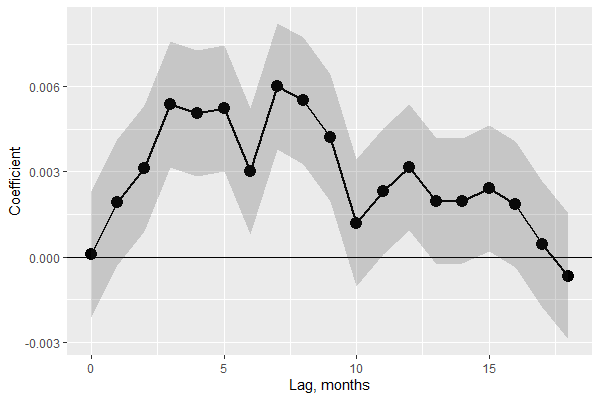
\includegraphics[width=0.95\textwidth]{paper_nov20/mPred_w.png}
\end{center}
\end{frame}


\begin{frame}
\begin{table}[!htbp] \centering 
  \caption*{Table 30: Predictability of industry employment by industry returns at semiannually frequency} 
  \label{} 
\begin{tabular}{@{\extracolsep{5pt}}lccc} 
\\[-1.8ex]\hline 
\hline \\[-1.8ex] 
 & \multicolumn{3}{c}{\textit{Dependent variable: Employment growth}} \\ 
\cline{2-4} 
\\[-1.8ex] & (1) & (2) & (3)\\ 
\hline \\[-1.8ex] 
 Return_{t-1} & 0.026$^{***}$ & 0.051$^{***}$ & 0.014$^{**}$ \\ 
  & (0.004) & (0.010) & (0.007) \\ 
  & & & \\ 
 Constant & $-$0.210$^{***}$ & $-$0.008 & $-$0.126 \\ 
  & (0.046) & (0.102) & (0.087) \\ 
  & & & \\ 
\hline \\[-1.8ex] 
Sample & Full & Negative R_{t-1} & Positive R_{t-1} \\
Observations & 826 & 419 & 407 \\ 
Adjusted R$^{2}$ & 0.046 & 0.055 & 0.007 \\ 
\hline 
\hline \\[-1.8ex] 
\end{tabular} 
\end{table}    
\end{frame}



\begin{frame}{Sectoral shifts hypothesis}
\begin{itemize}
    \item {Lilien(1982): Unemployment is driven by two types of shocks:}
    \begin{itemize}
        \item {Aggregate shocks.}
        \item {Reallocation shocks.}
    \end{itemize}
    \item {Aggregate shocks represent short-term fluctuations in business activity, while reallocation shocks reflect persistent changes in sectoral composition of the economy.}
    \item {While aggregate shocks have transitory effect on unemployment, reallocation shocks are more long-term in nature.}
    \item {Lilien (1982), Loungani et al.(1990) and Brainard et al.(1993): the variance in employment growth across industries predict aggregate unemployment growth at the annual frequency.}
\end{itemize}
\end{frame}


\scriptsize
{\renewcommand{\arraystretch}{0.96}
\begin{frame}{Unemployment predictability}
\begin{table}[!htbp] \centering 
  \caption*{\textbf{Table 13: Predictive regressions for unemployment}} 
  \vspace{-0.2cm}
\begin{tabular}{@{\extracolsep{5pt}}lcccccc} 
\\[-1.8ex]\hline 
\hline \\[-1.8ex] 
 & \multicolumn{6}{c}{\textit{Dependent variable:}} \\ 
\cline{2-7} 
 & \multicolumn{2}{c}{Unemployment} & \multicolumn{2}{c}{LT Unemployment} & \multicolumn{2}{c}{ST Unemployment} \\ 
\\[-1.8ex] & (1) & (2) & (3) & (4) & (5) & (6)\\ 
\hline \\[-1.8ex] 
 CID & 4.01$^{***}$ & 3.95$^{***}$ & 2.65$^{**}$ & 2.88$^{***}$ & 1.22$^{*}$ & 0.90 \\ 
  & [2.77] & [2.88] & [2.15] & [2.62] & [1.79] & [1.59] \\ 
  & & & & & & \\ 
 Mkt &  & $-$0.82$^{***}$ &  & $-$0.03 &  & $-$0.80$^{***}$ \\ 
  &  & [$-$2.58] &  & [$-$0.15] &  & [$-$4.11] \\ 
  & & & & & & \\ 
 Vol &  & 0.18$^{**}$ &  & 0.10$^{**}$ &  & 0.07$^{*}$ \\ 
  &  & [2.40] &  & [2.18] &  & [1.88] \\ 
  & & & & & & \\ 
 Constant & 0.004 & $-$0.01 & 0.01 & $-$0.002 & $-$0.002 & $-$0.01 \\ 
  & [0.09] & [$-$0.27] & [0.19] & [$-$0.07] & [$-$0.08] & [$-$0.49] \\ 
  & & & & & & \\ 
\hline \\[-1.8ex] 
Observations & 286 & 220 & 286 & 220 & 286 & 220 \\ 
R$^{2}$ & 0.03 & 0.19 & 0.05 & 0.14 & 0.01 & 0.18 \\ 
Adjusted R$^{2}$ & 0.03 & 0.18 & 0.04 & 0.13 & 0.004 & 0.17 \\ 
\hline 
\hline \\[-1.8ex] 
\end{tabular} 
\end{table}
\end{frame}
}


\normalsize
\begin{frame}{Interpretation of predictive regressions}
    \begin{itemize}
        \item {CID is a proxy for sectoral shifts, while aggregate market returns and volatility proxy for aggregate shocks.}
        \item {Long-term unemployment is predictable by CID and market volatility.}
        \item {Short-term unemployment is not predictable by CID, but is strongly predictable by first two moments of market returns.}
        \item {The results are consistent with sectoral shifts hypothesis of unemployment:}
        \begin{itemize}
            \item {Sectoral shifts shocks predicts long-term unemployment, but not short-term unemployment.}
            \item {Aggregate shocks predict short-term unemployment stronger than long-term unemployment.}
        \end{itemize}
    \end{itemize}
\end{frame}



\section{Additional Results}
\subsection{}


\normalsize
\begin{frame}{CID vs WID}
\begin{itemize}
    \item {Verousis and Voukelatos (2018) find that high sensitivity to cross-sectional dispersion (CSD) predicts low returns.}
    \item {Are their results driven by across- or within-industry dispersion?}
\end{itemize}
\scriptsize
\begin{table}[!htbp] \centering 
  \caption*{\textbf{Table 8: Abnormal returns of 5x5 portfolios, double-sorted on within-industry dispersion $\beta_{WID}$ and $\beta_{CID}$}} 
  \label{} 
\begin{tabular}{@{\extracolsep{5pt}} lcccccc} 
\\[-1.8ex]\hline 
\hline \\[-1.8ex] 
Statistic & Ret & $\alpha_{CAPM}$ & $\alpha_{FF3}$ & $\alpha_{Carhart}$ & $\alpha_{FF5}$ & $\alpha_{FF5+UMD+STR}$ \\ 
\hline \\[-1.8ex] 
L/S WID & 0.07 & 0.32$^{*}$ & 0.20 & 0.21 & -0.15 & -0.10 \\ 
T-stat & [ 0.40] & [ 1.74] & [ 1.22] & [ 1.28] & [ -0.97] & [ -0.63] \\ 
L/S CID & 0.30$^{**}$ & 0.23 & 0.14 & 0.27$^{*}$ & 0.20 & 0.28$^{**}$ \\ 
T-stat & [ 2.22] & [ 1.58] & [ 1.02] & [ 1.91] & [ 1.42] & [ 1.97] \\ 
\hline \\[-1.8ex] 
\end{tabular} 
\end{table}
\end{frame}


\normalsize
\begin{frame}{CID and CIV}
\begin{itemize}
    \item {Herskovic, Kelly, Lustig and Van Nieuwerburgh (2016) document existence of strong factor structure in idiosyncratic volatility of stock returns as well as fundamentals.}
    \item {Stocks with high exposure to common idiosyncratic volatility (CIV) earn small returns.}
    \item {They suggest a variation of the model of Constantinides and Duffie (1996) to motivate CIV as household income risk.}
    \item {How is CID different from CIV?}
\end{itemize}

\end{frame}


\footnotesize
\begin{frame}{CID and CIV: double-sorts}
\begin{table}[!htbp] \centering 
  \caption*{\textbf{Table 11: Abnormal returns of 5x5 portfolios, double-sorted on $\beta_{CID}$ and $\beta_{CIV}$}}
  \label{} 
  \begin{flushleft}
    {\medskip \scriptsize
 The table reports abnormal monthly returns of long-short value-weighted portfolios, formed from independent 5 by 5 double sorts on $\beta_{CID}$ and $\beta_{CIV}$. CIV is common idiosyncratic volatility from Herskovic, Kelly, Lustig and Van Nieuwerburgh (2016). }
    \medskip
    \end{flushleft}
\begin{tabular}{@{\extracolsep{5pt}} lcccccc} 
\\[-1.8ex]\hline 
\hline \\[-1.8ex] 
Statistic & Ret & $\alpha_{CAPM}$ & $\alpha_{FF3}$ & $\alpha_{Carhart}$ & $\alpha_{FF5}$ & $\alpha_{FF5+UMD+STR}$ \\ 
\hline \\[-1.8ex] 
L/S CIV & 0.08 & -0.01 & -0.01 & -0.05 & 0.05 & 0.01 \\ 
T-stat & [ 0.57] & [ -0.07] & [ -0.10] & [ -0.37] & [ 0.39] & [ 0.04] \\
L/S CID & 0.40$^{***}$ & 0.43$^{***}$ & 0.28$^{**}$ & 0.54$^{***}$ & 0.20 & 0.43$^{***}$ \\ 
T-stat & [ 2.78] & [ 2.94] & [ 2.02] & [ 4.02] & [ 1.40] & [ 3.16] \\ 
\hline \\[-1.8ex] 
\end{tabular} 
\end{table}
\end{frame}



\scriptsize
{\renewcommand{\arraystretch}{0.52}
\begin{frame}{CID and CIV: Spanning tests between the two factors}
\vspace{-0.3cm}
\begin{table}[!htbp] \centering 
\begin{tabular}{@{\extracolsep{5pt}}lcccc} 
\\[-1.8ex]\hline 
\hline \\[-1.8ex] 
 & \multicolumn{4}{c}{\textit{Dependent variable:}} \\ 
\cline{2-5} 
\\[-1ex] & \multicolumn{2}{c}{CID factor} & \multicolumn{2}{c}{CIV factor} \\ 
\\[-1.8ex] & (1) & (2) & (3) & (4)\\ 
%\vspace{0.3cm}
\hline \\[-0.5ex] 
 EMKT & 0.033 & 0.066$^{*}$ & $-$0.154$^{***}$ & $-$0.160$^{***}$ \\ 
  & [0.926] & [1.865] & [$-$4.354] & [$-$4.651] \\ 
  & & & & \\ 
 SMB & $-$0.076 & $-$0.027 & $-$0.231$^{***}$ & $-$0.215$^{***}$ \\ 
  & [$-$1.479] & [$-$0.519] & [$-$4.520] & [$-$4.292] \\ 
  & & & & \\ 
 HML & $-$0.191$^{***}$ & $-$0.164$^{**}$ & $-$0.129$^{*}$ & $-$0.088 \\ 
  & [$-$2.667] & [$-$2.328] & [$-$1.805] & [$-$1.258] \\ 
  & & & & \\ 
 RMW & $-$0.227$^{***}$ & $-$0.205$^{***}$ & $-$0.102 & $-$0.054 \\ 
  & [$-$3.206] & [$-$2.957] & [$-$1.453] & [$-$0.780] \\ 
  & & & & \\ 
 CMA & $-$0.131 & $-$0.157 & 0.117 & 0.145 \\ 
  & [$-$1.243] & [$-$1.513] & [1.119] & [1.413] \\ 
  & & & & \\ 
 MOM & 0.284$^{***}$ & 0.270$^{***}$ & 0.067$^{**}$ & 0.007 \\ 
  & [8.289] & [8.020] & [1.977] & [0.205] \\ 
  & & & & \\ 
 CIVf &  & 0.215$^{***}$ &  &  \\ 
  &  & [5.326] &  &  \\ 
  & & & & \\ 
 CIDf &  &  &  & 0.211$^{***}$ \\ 
  &  &  &  & [5.326] \\ 
  & & & & \\ 
 Constant & $-$0.501$^{***}$ & $-$0.468$^{***}$ & $-$0.152 & $-$0.046 \\ 
  & [$-$3.392] & [$-$3.239] & [$-$1.040] & [$-$0.321] \\ 
  & & & & \\ 
\hline \\[-1.2ex] 
Observations & 605 & 605 & 605 & 605 \\ 
Adjusted R$^{2}$ & 0.166 & 0.202 & 0.093 & 0.133 \\ 
\hline 
\hline \\[-1.8ex]
\end{tabular} 
\end{table}
\end{frame}
}
\footnotesize


\scriptsize
\begin{frame}{CID and volatility measures}
\begin{table}[!htbp] \centering 
  \caption*{\textbf{Table 10: Abnormal returns of 5x5 portfolios, double-sorted on $\beta_{CID}$ and sensitivity to other variables}}
\begin{tabularx}{\linewidth}{p{1.5cm}p{1.2cm}p{1.2cm}p{1.2cm}p{1.2cm}p{1.2cm}p{1.2cm}}
    \toprule
    \multicolumn{7}{l}{\textbf{Panel A: Market volatility vs CID}} \\
    \midrule 
\\[-1.8ex]\hline 
\hline \\[-1.8ex] 
Statistic & Ret & $\alpha_{CAPM}$ & $\alpha_{FF3}$ & $\alpha_{Carhart}$ & $\alpha_{FF5}$ & $\alpha_{FF5+UMD+STR}$ \\ 
\hline \\[-1.8ex] 
L/S VOL & 0.26$^{*}$ & 0.14 & 0.19 & 0.22 & 0.38$^{***}$ & 0.36$^{***}$ \\ 
T-stat & [ 1.87] & [ 1.06] & [ 1.42] & [ 1.61] & [ 2.80] & [ 2.61] \\ 
L/S CID & 0.42$^{***}$ & 0.47$^{***}$ & 0.38$^{***}$ & 0.60$^{***}$ & 0.34$^{**}$ & 0.52$^{***}$ \\ 
T-stat & [ 3.09] & [ 3.43] & [ 2.82] & [ 4.55] & [ 2.41] & [ 3.81] \\ 
\hline \\[-1.8ex]
\end{tabularx}



\begin{tabularx}{\linewidth}{p{1.5cm}p{1.2cm}p{1.2cm}p{1.2cm}p{1.2cm}p{1.2cm}p{1.2cm}}
    \toprule
    \multicolumn{7}{l}{\textbf{Panel D: NVIX vs CID}} \\
    \midrule  
\\[-1.8ex]\hline 
\hline \\[-1.8ex] 
Statistic & Ret & $\alpha_{CAPM}$ & $\alpha_{FF3}$ & $\alpha_{Carhart}$ & $\alpha_{FF5}$ & $\alpha_{FF5+UMD+STR}$ \\ 
\hline \\[-1.8ex] 
L/S NVIX & 0.04 & -0.10 & -0.03 & 0.06 & 0.25$^{*}$ & 0.36$^{***}$ \\ 
T-stat & [ 0.26] & [ -0.72] & [ -0.19] & [ 0.42] & [ 1.88] & [ 2.63] \\ 
L/S CID & 0.45$^{***}$ & 0.49$^{***}$ & 0.33$^{**}$ & 0.55$^{***}$ & 0.23 & 0.43$^{***}$ \\ 
T-stat & [ 2.99] & [ 3.26] & [ 2.28] & [ 3.82] & [ 1.54] & [ 2.94] \\ 
\hline \\[-1.8ex] 
\end{tabularx} 
\end{table} 
\end{frame}



\begin{frame}{CID and uncertainty measures}
\begin{table}[!htbp] \centering 
  \caption*{\textbf{Table 10: Abnormal returns of 5x5 portfolios, double-sorted on $\beta_{CID}$ and sensitivity to other variables}}
  \label{} 
  \vspace{-0.3cm}
  \begin{flushleft}
    {\medskip
    \scriptsize
 MU and FU are macroeconomic/financial uncertainty from Ludvigson et al. (2015).}
    \medskip
    \end{flushleft}

\begin{tabularx}{\linewidth}{p{1.5cm}p{1.2cm}p{1.2cm}p{1.2cm}p{1.2cm}p{1.2cm}p{1.2cm}}
    \toprule
    \multicolumn{7}{l}{\textbf{Panel C: Financial uncertainty (Ludvigson 2015) vs CID}} \\
    \midrule 
\\[-1.8ex]\hline 
\hline \\[-1.8ex] 
Statistic & Ret & $\alpha_{CAPM}$ & $\alpha_{FF3}$ & $\alpha_{Carhart}$ & $\alpha_{FF5}$ & $\alpha_{FF5+UMD+STR}$ \\ 
\hline \\[-1.8ex] 
L/S FU & -0.04 & -0.16 & -0.29$^{**}$ & -0.40$^{***}$ & -0.41$^{***}$ & -0.48$^{***}$ \\ 
T-stat & [ -0.30] & [ -1.10] & [ -2.07] & [ -2.89] & [ -2.91] & [ -3.33] \\ 
L/S CID & 0.44$^{***}$ & 0.49$^{***}$ & 0.39$^{***}$ & 0.67$^{***}$ & 0.41$^{***}$ & 0.65$^{***}$ \\ 
T-stat & [ 3.33] & [ 3.66] & [ 2.97] & [ 5.34] & [ 3.02] & [ 5.08] \\ 
\hline \\[-1.8ex] 
\end{tabularx} 

\begin{tabularx}{\linewidth}{p{1.5cm}p{1.2cm}p{1.2cm}p{1.2cm}p{1.2cm}p{1.2cm}p{1.2cm}}
    \toprule
    \multicolumn{7}{l}{\textbf{Panel B: Macroeconomic uncertainty (Ludvigson 2015) vs CID}} \\
    \midrule  
\\[-1.8ex]\hline 
\hline \\[-1.8ex] 
Statistic & Ret & $\alpha_{CAPM}$ & $\alpha_{FF3}$ & $\alpha_{Carhart}$ & $\alpha_{FF5}$ & $\alpha_{FF5+UMD+STR}$ \\ 
\hline \\[-1.8ex] 
L/S MU & -0.16 & -0.26$^{*}$ & -0.22 & -0.17 & 0.00 & -0.07 \\ 
T-stat & [ -1.09] & [ -1.83] & [ -1.58] & [ -1.25] & [ 0.02] & [ -0.51] \\ 
L/S CID & 0.41$^{***}$ & 0.43$^{***}$ & 0.28$^{**}$ & 0.54$^{***}$ & 0.18 & 0.41$^{***}$ \\ 
T-stat & [ 2.83] & [ 2.97] & [ 1.96] & [ 3.98] & [ 1.24] & [ 3.00] \\ 
\hline \\[-1.8ex] 
\end{tabularx} 
\end{table} 
\end{frame}


\begin{frame}{Other industry classifications}
{Figure 3}
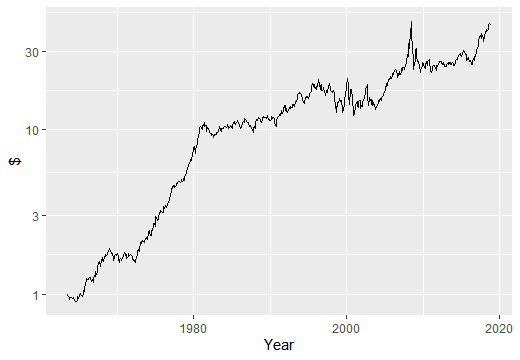
\includegraphics[width=0.94\textwidth]{Figure3_sl.png}
\end{frame}



\section{Conclusion}
\subsection{}


\normalsize
\begin{frame}{Conclusion}
\begin{itemize}
    \item {Stocks with high sensitivity to CID produce low returns.}
    \item {The long-short strategy, based on $\beta_{CID}$, delivers 29-63 bps of monthly abnormal returns.}
    \item {High $\beta_{CID}$ stocks are likely to benefit from sectoral shifts and thus are less risky.}
    \item {CID subsumes a large fraction of CIV premium.}
    \item {High innovations in CID predict high unemployment growth.}
    \item {Results are consistent with CID proxying for unemployment risk from sectoral shifts.}
\end{itemize}
\end{frame}


\section{Appendix}
\subsection{}


\scriptsize
\begin{frame}{Factor loadings of quintile portfolios, formed on $\beta_{CID}$}
\vspace{-0.25cm}
\begin{table}[!htbp] \centering 
  \label{} 
\begin{tabular}{@{\extracolsep{-8pt}} ccccccccccc} 
\\[-1.8ex]\hline 
\hline \\[-1.8ex] 
Quintile & Ret & $\alpha$ & EMKT & HML & SMB & RMW & CMA & MOM & STR & adjR2 \\ 
\hline \\[-1.8ex] 
1 & 0.79 & 0.27 & 1.07 & 0.10 & 0.17 & 0.06 & -0.01 & -0.16 & -0.01 & 0.85 \\ 
 & [ 3.83] & [ 3.07] & [ 49.36] & [ 2.34] & [ 5.78] & [ 1.50] & [ -0.16] & [ -7.44] & [ -0.29] &  \\ 
2 & 0.63 & 0.07 & 1.02 & 0.13 & -0.01 & 0.19 & 0.08 & -0.12 & 0.02 & 0.90 \\ 
 & [ 3.51] & [ 1.08] & [ 67.00] & [ 4.46] & [ -0.49] & [ 6.32] & [ 1.89] & [ -8.30] & [ 0.86] &  \\ 
3 & 0.58 & 0.03 & 0.97 & 0.05 & -0.07 & 0.18 & 0.11 & -0.05 & 0.01 & 0.94 \\ 
 & [ 3.55] & [ 0.64] & [ 91.19] & [ 2.27] & [ -4.64] & [ 8.87] & [ 3.79] & [ -5.02] & [ 0.87] &  \\ 
4 & 0.45 & -0.09 & 0.99 & -0.04 & -0.05 & 0.06 & 0.04 & 0.02 & 0.03 & 0.92 \\ 
 & [ 2.59] & [ -1.72] & [ 78.18] & [ -1.47] & [ -2.82] & [ 2.32] & [ 1.00] & [ 1.47] & [ 1.77] &  \\ 
5 & 0.30 & -0.23 & 1.11 & -0.04 & 0.08 & -0.28 & -0.18 & 0.13 & 0.00 & 0.87 \\ 
 & [ 1.40] & [ -2.72] & [ 53.56] & [ -0.95] & [ 2.70] & [ -7.08] & [ -3.09] & [ 6.54] & [ -0.11] &  \\ 
L/S & -0.49 & -0.50 & 0.04 & -0.14 & -0.10 & -0.35 & -0.17 & 0.29 & 0.01 & 0.14 \\ 
 & [ -3.19] & [ -3.26] & [ 0.93] & [ -1.87] & [ -1.85] & [ -4.75] & [ -1.60] & [ 7.88] & [ 0.11] &  \\ 
\hline \\[-1.8ex] 
\end{tabular} 
\end{table}
\end{frame}


\begin{frame}{CID vs WID using FF5 industry classification}
\begin{table}[!htbp] \centering 
  \caption*{\textbf{Table 16: Abnormal returns of 5x5 portfolios, double-sorted on within-industry dispersion $\beta_{WID}$ and $\beta_{CID}$} using FF5 industry classification} 
  \label{} 
  \begin{flushleft}
    {\medskip\scriptsize
 The table reports abnormal monthly returns of long-short value-weighted portfolios, formed from independent 5 by 5 double sorts on $\beta_{WID}$ and $\beta_{CID}$. WID (within-industry dispersion) is a mean absolute deviation of returns of the stocks within each industry, averaged across 5 industries.}
    \medskip
    \end{flushleft}
\begin{tabular}{@{\extracolsep{5pt}} ccccccc} 
\\[-1.8ex]\hline 
\hline \\[-1.8ex] 
Statistic & Ret & $\alpha_{CAPM}$ & $\alpha_{FF3}$ & $\alpha_{Carhart}$ & $\alpha_{FF5}$ & $\alpha_{FF5+UMD+STR}$ \\ 
\hline \\[-1.8ex] 
L/S WID & 0.10 & 0.30$^{**}$ & 0.23$^{*}$ & 0.16 & -0.02 & -0.05 \\ 
T-stat & [ 0.61] & [ 2.03] & [ 1.72] & [ 1.20] & [ -0.13] & [ -0.39] \\
L/S CID & 0.17 & 0.13 & -0.01 & 0.27$^{***}$ & 0.09 & 0.27$^{**}$ \\ 
T-stat & [ 1.44] & [ 1.14] & [ -0.08] & [ 2.63] & [ 0.77] & [ 2.54] \\ 
\hline \\[-1.8ex]
\end{tabular} 
\end{table}
\end{frame}



\scriptsize
\renewcommand{\arraystretch}{0.88}
\begin{frame}{Unemployment predictability}
% Table created by stargazer v.5.2.2 by Marek Hlavac, Harvard University. E-mail: hlavac at fas.harvard.edu
% Date and time: Wed, Jun 10, 2020 - 2:32:51 PM
\begin{table}[!htbp] \centering 
  \label{} 
\begin{tabular}{@{\extracolsep{5pt}}lccc} 
\\[-1.8ex]\hline 
\hline \\[-1.8ex] 
 & \multicolumn{3}{c}{\textit{Dependent variable: Unemployment growth}} \\ 
\cline{2-4} 
\\[-1.8ex] & (1) & (2) & (3)\\ 
\hline \\[-1.8ex] 
 CIV & 4.02$^{***}$ & 3.97$^{***}$ & 3.69$^{***}$ \\ 
  & [2.77] & [2.90] & [2.85] \\ 
  & & & \\ 
 Mkt &  & $-$0.80$^{**}$ & $-$0.71$^{**}$ \\ 
  &  & [$-$2.53] & [$-$2.34] \\ 
  & & & \\ 
 Vol &  & 0.17$^{**}$ & 0.17$^{**}$ \\ 
  &  & [2.37] & [2.51] \\ 
  & & & \\ 
 FU &  &  & 0.83 \\ 
  &  &  & [0.60] \\ 
  & & & \\ 
 CIV &  &  & 0.02 \\ 
  &  &  & [0.37] \\ 
  & & & \\ 
 Constant & 0.005 & $-$0.01 & $-$0.01 \\ 
  & [0.10] & [$-$0.27] & [$-$0.27] \\ 
  & & & \\ 
\hline \\[-1.8ex] 
Observations & 284 & 220 & 220 \\ 
R$^{2}$ & 0.03 & 0.19 & 0.19 \\ 
Adjusted R$^{2}$ & 0.03 & 0.18 & 0.17 \\ 
\hline 
\hline \\[-1.8ex] 
\end{tabular} 
\end{table} 
\end{frame}


\scriptsize
\begin{frame}{Long-term unemployment predictability}
\begin{table}[!htbp] \centering 
  \label{} 
\begin{tabular}{@{\extracolsep{5pt}}lccc} 
\\[-1.8ex]\hline 
\hline \\[-1.8ex] 
 & \multicolumn{3}{c}{\textit{Dependent variable: Long-term unemployment growth}} \\ 
\cline{2-4} 
\\[-1.8ex] & (1) & (2) & (3)\\ 
\hline \\[-1.8ex] 
 CID & 2.65$^{**}$ & 2.88$^{***}$ & 3.22$^{***}$ \\ 
  & [2.15] & [2.62] & [3.14] \\ 
  & & & \\ 
 Mkt &  & $-$0.03 & $-$0.12 \\ 
  &  & [$-$0.14] & [$-$0.56] \\ 
  & & & \\ 
 Vol &  & 0.10$^{**}$ & 0.11$^{**}$ \\ 
  &  & [2.16] & [2.34] \\ 
  & & & \\ 
 FU &  &  & $-$0.21 \\ 
  &  &  & [$-$0.25] \\ 
  & & & \\ 
 CIV &  &  & $-$0.04 \\ 
  &  &  & [$-$0.91] \\ 
  & & & \\ 
 Constant & 0.01 & $-$0.002 & $-$0.002 \\ 
  & [0.19] & [$-$0.07] & [$-$0.08] \\ 
  & & & \\ 
\hline \\[-1.8ex] 
Observations & 284 & 220 & 220 \\ 
R$^{2}$ & 0.05 & 0.14 & 0.14 \\ 
Adjusted R$^{2}$ & 0.04 & 0.13 & 0.13 \\ 
\hline 
\hline \\[-1.8ex] 
\end{tabular} 
\end{table}
\end{frame}


\scriptsize
\begin{frame}{Short-term unemployment predictability}
\begin{table}[!htbp] \centering 
  \label{} 
\begin{tabular}{@{\extracolsep{5pt}}lccc} 
\\[-1.8ex]\hline 
\hline \\[-1.8ex] 
 & \multicolumn{3}{c}{\textit{Dependent variable: Short-term unemployment growth}} \\
\cline{2-4} 
\\[-1.8ex] & (1) & (2) & (3)\\ 
\hline \\[-1.8ex] 
 CID & 1.22$^{*}$ & 0.90 & 0.14 \\ 
  & [1.79] & [1.59] & [0.21] \\ 
  & & & \\ 
 Mkt &  & $-$0.80$^{***}$ & $-$0.57$^{***}$ \\ 
  &  & [$-$4.11] & [$-$3.49] \\ 
  & & & \\ 
 Vol &  & 0.07$^{*}$ & 0.06 \\ 
  &  & [1.88] & [1.64] \\ 
  & & & \\ 
 FU &  &  & 1.25 \\ 
  &  &  & [1.56] \\ 
  & & & \\ 
 CIV &  &  & 0.07$^{*}$ \\ 
  &  &  & [1.92] \\ 
  & & & \\ 
 Constant & $-$0.002 & $-$0.01 & $-$0.01 \\ 
  & [$-$0.08] & [$-$0.49] & [$-$0.45] \\ 
  & & & \\ 
\hline \\[-1.8ex] 
Observations & 286 & 220 & 220 \\ 
R$^{2}$ & 0.01 & 0.18 & 0.21 \\ 
Adjusted R$^{2}$ & 0.004 & 0.17 & 0.19 \\ 
\hline 
\hline \\[-1.8ex] 
\end{tabular} 
\end{table}
\end{frame}


\renewcommand{\arraystretch}{1.00}


\scriptsize
{\renewcommand{\arraystretch}{0.72}
\begin{frame}{Appendix: Fama-MacBeth across stocks}
\vspace{-0.38cm}
\begin{table}[!htbp] \centering 
\begin{tabular}{@{\extracolsep{0pt}}lccccccc} 
\\[-1.8ex]\hline 
\hline \\[-1.8ex] 
 & \multicolumn{7}{c}{\textit{Dependent variable: Return}} \\ 
\cline{2-8} 
\\[-1.8ex] & (1) & (2) & (3) & (4) & (5) & (6) & (7)\\ 
\hline \\[-1.8ex] 
 $\beta_{CID}$ & $-$0.05$^{**}$ & $-$0.03$^{*}$ & $-$0.02$^{*}$ & $-$0.02$^{*}$ & $-$0.02$^{**}$ & $-$0.02$^{**}$ & $-$0.02$^{**}$ \\ 
  & [$-$2.29] & [$-$1.87] & [$-$1.80] & [$-$1.72] & [$-$2.02] & [$-$2.00] & [$-$2.09] \\ 
  & & & & & & & \\ 
 $\beta$ &  & $-$0.21 & $-$0.20 & $-$0.07 & $-$0.29 & $-$0.23 & 0.13 \\ 
  &  & [$-$0.75] & [$-$0.63] & [$-$0.25] & [$-$1.00] & [$-$0.78] & [0.46] \\ 
  & & & & & & & \\ 
 size &  &  & $-$0.05 & $-$0.03 & $-$0.02 & $-$0.03 & $-$0.09$^{**}$ \\ 
  &  &  & [$-$1.15] & [$-$0.71] & [$-$0.51] & [$-$0.68] & [$-$2.38] \\ 
  & & & & & & & \\ 
 logbm &  &  &  & 0.22$^{***}$ & 0.22$^{***}$ & 0.15$^{***}$ & 0.11$^{**}$ \\ 
  &  &  &  & [3.83] & [3.93] & [2.68] & [2.12] \\ 
  & & & & & & & \\ 
 mom122 &  &  &  &  & 1.33$^{***}$ & 1.26$^{***}$ & 1.13$^{***}$ \\ 
  &  &  &  &  & [7.08] & [6.63] & [6.06] \\ 
  & & & & & & & \\ 
 inv &  &  &  &  &  & $-$0.94$^{***}$ & $-$0.93$^{***}$ \\ 
  &  &  &  &  &  & [$-$6.79] & [$-$6.76] \\ 
  & & & & & & & \\ 
 MAX &  &  &  &  &  &  & $-$0.08$^{***}$ \\ 
  &  &  &  &  &  &  & [$-$12.34] \\ 
  & & & & & & & \\ 
 Constant & 0.66$^{***}$ & 0.84$^{***}$ & 1.05$^{***}$ & 2.44$^{***}$ & 2.44$^{***}$ & 2.01$^{***}$ & 2.20$^{***}$ \\ 
  & [3.49] & [4.80] & [4.30] & [5.51] & [5.57] & [4.63] & [5.05] \\ 
  & & & & & & & \\ 
\hline \\[-1.8ex] 
Adjusted R$^{2}$ & 0.0001 & 0.0003 & 0.0003 & 0.001 & 0.001 & 0.001 & 0.002 \\ 
\hline 
\hline \\[-1.8ex] 
\end{tabular}
\end{table}
\end{frame}
}



\scriptsize
\begin{frame}{Appendix: CID, constructed from abnormal industry returns}
\begin{table}[!htbp] \centering 
  \caption{\textbf{Returns of the quintile portfolios, formed on $\beta_{CID}$, calculated from abnormal returns of FF49 industry portfolios}} 
  \label{} 
  \vspace{-0.4cm}
\begin{tabular}{@{\extracolsep{5pt}} ccccccc} 
\\[-1.8ex]\hline 
\hline \\[-1.8ex] 
 & Q1 & Q2 & Q3 & Q4 & Q5 & L/S \\ 
\hline \\[-1.8ex] 
Mean ew & 0.76$^{***}$ & 0.79$^{***}$ & 0.72$^{***}$ & 0.68$^{***}$ & 0.52$^{**}$ & -0.24$^{**}$ \\ 
T-stat ew & [3.45] & [4.20] & [3.96] & [3.51] & [2.15] & [-2.17] \\ 
Mean vw & 0.78$^{***}$ & 0.63$^{***}$ & 0.51$^{***}$ & 0.53$^{***}$ & 0.31 & -0.48$^{***}$ \\ 
T-stat vw & [3.94] & [3.70] & [3.15] & [3.10] & [1.37] & [-3.20] \\ 
\hline \\[-1.8ex] 
\end{tabular}
\end{table}



% Table created by stargazer v.5.2.2 by Marek Hlavac, Harvard University. E-mail: hlavac at fas.harvard.edu
% Date and time: Sat, Sep 14, 2019 - 4:34:17 PM
\begin{table}[!htbp] \centering 
  \caption{\textbf{Abnormal returns of the long-short portfolio, formed on $\beta_{CID}$, calculated from abnormal returns of FF49 industry portfolios}} 
  \label{} 
  \vspace{-0.4cm}
\begin{tabular}{@{\extracolsep{5pt}} ccccccc} 
\\[-1.8ex]\hline 
\hline \\[-1.8ex] 
Statistic & Ret & $\alpha_{CAPM}$ & $\alpha_{FF3}$ & $\alpha_{Carhart}$ & $\alpha_{FF5}$ & $\alpha_{FF5+UMD+STR}$ \\ 
\hline \\[-1.8ex] 
L/S & -0.48$^{***}$ & -0.55$^{***}$ & -0.44$^{***}$ & -0.57$^{***}$ & -0.22 & -0.30$^{**}$ \\ 
 & [-3.20] & [-3.69] & [-2.97] & [-3.84] & [-1.47] & [-2.04] \\   
\hline \\[-1.8ex] 
\end{tabular} 
\end{table}
\end{frame}



\begin{frame}{Appendix: 2x3 Double-sort on $\beta_{CID}$ and size}
\begin{table}[!htbp] \centering 
  \caption{\textbf{Abnormal returns of 2x3 portfolios, double-sorted on size and $\beta_{CID}$}}
  \label{} 
\begin{tabular}{@{\extracolsep{5pt}} lcccccc} 
\\[-1.8ex]\hline 
\hline \\[-1.8ex] 
Statistic & Ret & $\alpha_{CAPM}$ & $\alpha_{FF3}$ & $\alpha_{Carhart}$ & $\alpha_{FF5}$ & $\alpha_{FF5+UMD+STR}$ \\ 
\hline \\[-1.8ex] 
L/S Size & 0.21$^{**}$ & 0.14 & -0.04 & 0.01 & -0.07$^{**}$ & -0.05$^{*}$ \\ 
T-stat & [ 2.11] & [ 1.45] & [ -1.15] & [ 0.36] & [ -2.24] & [ -1.66] \\ 
L/S CID & 0.28$^{***}$ & 0.30$^{***}$ & 0.20$^{**}$ & 0.40$^{***}$ & 0.17$^{*}$ & 0.33$^{***}$ \\ 
T-stat & [ 2.72] & [ 2.94] & [ 2.05] & [ 4.16] & [ 1.68] & [ 3.40] \\
\hline \\[-1.8ex] 
\end{tabular}
\end{table}
\end{frame}



\begin{frame}{Appendix: Performance of $\beta_{CID}$ strategy}
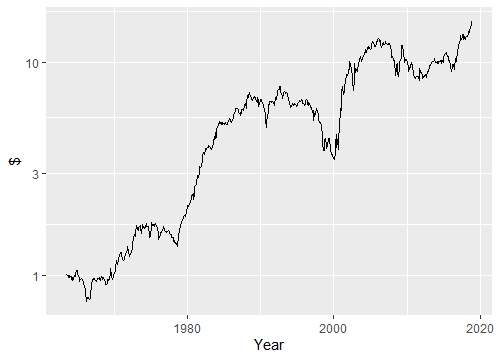
\includegraphics[width=1\textwidth]{Figure2_sl.png}    
\end{frame}



\begin{frame}{Appendix: Quintile portfolios of industry portfolios}

\begin{table}[!htbp] \centering 
  \caption{\textbf{Average returns of quintile $\beta_{CID}$-sorted portfolios, formed from 49 industry portfolios}} 
  \label{} 
\begin{tabular}{@{\extracolsep{5pt}} ccccccc} 
\\[-1.8ex]\hline 
\hline \\[-1.8ex] 
 & Q1 & Q2 & Q3 & Q4 & Q5 & L/S \\ 
\hline \\[-1.8ex] 
Mean ew & 0.98$^{***}$ & 0.91$^{***}$ & 0.96$^{***}$ & 0.92$^{***}$ & 0.84$^{***}$ & -0.14 \\ 
T-stat ew & [4.87] & [4.79] & [5.12] & [4.74] & [4.07] & [-1.06] \\ 
Mean vw & 1.09$^{***}$ & 0.86$^{***}$ & 1.04$^{***}$ & 0.85$^{***}$ & 0.78$^{***}$ & -0.31$^{*}$ \\ 
T-stat vw & [5.62] & [4.65] & [5.65] & [4.54] & [3.78] & [-1.90] \\ 
\hline \\[-1.8ex] 
\end{tabular} 
\end{table} 


\begin{table}[!htbp] \centering 
  \caption{\textbf{Abnormal returns of quintile $\beta_{CID}$-sorted portfolios, formed from 49 industry portfolios}} 
  \label{} 
\begin{tabular}{@{\extracolsep{0pt}} ccccccc} 
\\[-1.8ex]\hline 
\hline \\[-1.8ex] 
Statistic & Ret & $\alpha_{CAPM}$ & $\alpha_{FF3}$ & $\alpha_{Carhart}$ & $\alpha_{FF5}$ & $\alpha_{FF5+UMD+STR}$ \\ 
\hline \\[-1.8ex] 
L/S & -0.31$^{*}$ & -0.36$^{**}$ & -0.20 & -0.43$^{***}$ & -0.09 & -0.31$^{**}$ \\ 
 & [-1.92] & [-2.21] & [-1.32] & [-2.82] & [-0.57] & [-1.98] \\ 
\hline \\[-1.8ex] 
\end{tabular} 
\end{table}
\end{frame}


\begin{frame}{Daily frequency: Return spread}
\begin{table}[!htbp] \centering 
  \caption{Quintile abnormal returns using daily $\beta_{CID}$} 
  \label{} 
    \begin{flushleft}
    {\medskip\small
 The table reports abnormal monthly returns of the long-short value-weighted quintile portfolio, formed from sorts on $\beta_{CID}$. The last column contains the abnormal returns with respect to Fama-French 5 factor model, augmented with momentum and short-term reversal factors. The returns are calculated at the monthly frequency over 1963-2019.}
    \medskip
    \end{flushleft}
\begin{tabular}{@{\extracolsep{5pt}} ccccccc} 
\\[-1.8ex]\hline 
\hline \\[-1.8ex] 
Statistic & Ret & $\alpha_{CAPM}$ & $\alpha_{FF3}$ & $\alpha_{Carhart}$ & $\alpha_{FF5}$ & $\alpha_{FF5+UMD+STR}$ \\ 
\hline \\[-1.8ex] 
LS & -0.31$^{**}$ & -0.31$^{**}$ & -0.35$^{***}$ & -0.19 & -0.34$^{***}$ & -0.13 \\ 
 & [-2.29] & [-2.34] & [-2.75] & [-1.51] & [-2.61] & [-0.96] \\ 
\hline \\[-1.8ex] 
\end{tabular} 
\end{table}
\end{frame}



\begin{frame}{Daily frequency: preranking vs postranking betas}
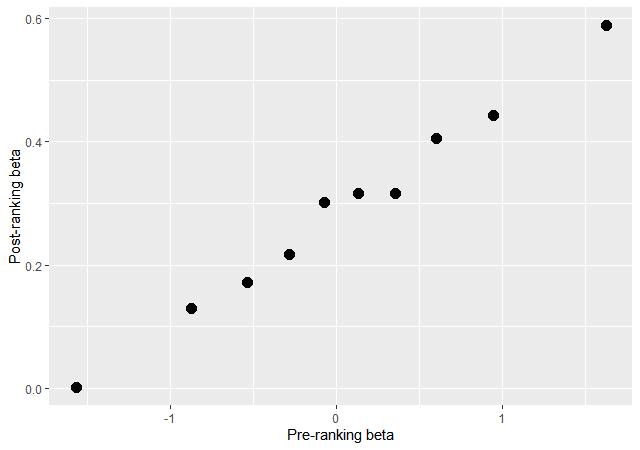
\includegraphics[width=0.88\textwidth]{paper_b3/Figure2_sl.png}
\end{frame}

\begin{frame}{Monthly-frequency: preranking vs postranking betas}
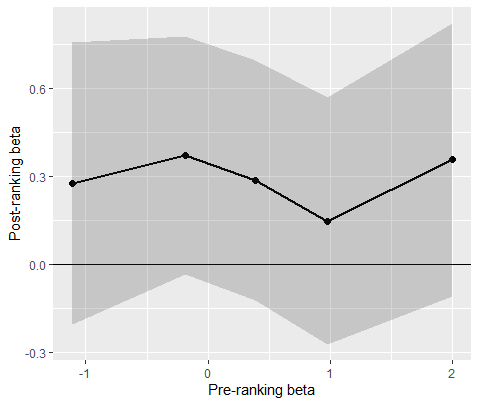
\includegraphics[width=0.8\textwidth]{betas_nov_0.png}
\end{frame}

\begin{frame}{Quarterly frequency: preranking vs postranking betas}
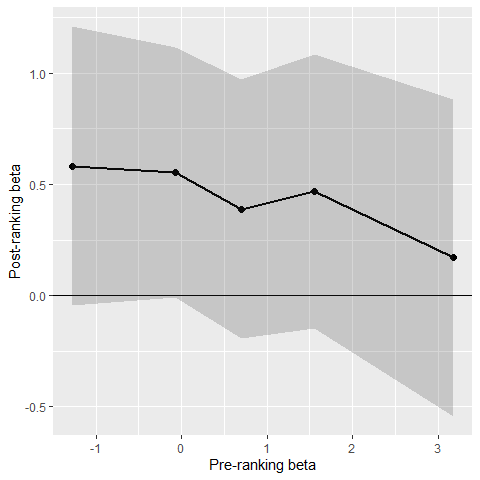
\includegraphics[width=0.64\textwidth]{paper_nov20/betas_qtr.png}
\end{frame}



\begin{frame}{Quarterly frequency: Return spread}
\begin{table}[!htbp] \centering 
  \caption{Quintile abnormal returns using quarterly $\beta_{CID}$} 
  \label{} 
    \begin{flushleft}
    {\medskip\small
 The table reports abnormal monthly returns of the long-short value-weighted quintile portfolio, formed from sorts on $\beta_{CID}$. The last column contains the abnormal returns with respect to Fama-French 5 factor model, augmented with momentum and short-term reversal factors. The returns are calculated at the monthly frequency over 1963-2019.}
    \medskip
    \end{flushleft}
\begin{tabular}{@{\extracolsep{5pt}} ccccccc} 
\\[-1.8ex]\hline 
\hline \\[-1.8ex] 
Statistic & Ret & $\alpha_{CAPM}$ & $\alpha_{FF3}$ & $\alpha_{Carhart}$ & $\alpha_{FF5}$ & $\alpha_{FF5+UMD+STR}$ \\ 
\hline \\[-1.8ex] 
LS & -0.22 & -0.29$^{**}$ & -0.19 & -0.38$^{***}$ & -0.24$^{*}$ & -0.40$^{***}$ \\ 
 & [-1.51] & [-2.06] & [-1.38] & [-2.86] & [-1.69] & [-2.90] \\ 
\hline \\[-1.8ex] 
\end{tabular} 
\end{table}    
\end{frame}


\begin{frame}{Correlations}
\begin{table}[!htbp] \centering 
  \caption{Correlations between L/S portfolios, formed on $\beta_{CID}$ at varying frequencies} 
  \label{} 
      \begin{flushleft}
    {\medskip\small
 The table reports abnormal monthly returns of the long-short value-weighted quintile portfolio, formed from sorts on $\beta_{CID}$. The last column contains the abnormal returns with respect to Fama-French 5 factor model, augmented with momentum and short-term reversal factors. The returns are calculated at the monthly frequency over 1963-2019.}
    \medskip
    \end{flushleft}
\begin{tabular}{@{\extracolsep{5pt}} ccc} 
\\[-1.8ex]\hline 
\hline \\[-1.8ex] 
Quarterly\_LS & Monthly\_LS & Daily\_LS \\ 
\hline \\[-1.8ex] 
$1$ & $0.26$ & $$-$0.04$ \\ 
$0.26$ & $1$ & $0.06$ \\ 
$$-$0.04$ & $0.06$ & $1$ \\ 
\hline \\[-1.8ex] 
\end{tabular} 
\end{table}  
\end{frame}


\end{document}

